\chapter{Sistemi di Crowdsourcing}
\label{chap:due}
Con il termine Crowdsourcing ci si riferisce alla \textit{possibilità di utilizzare i contributi indipendenti di una "folla" per uno scopo, senza che questi siano organizzati a priori in flussi di lavoro} \cite{book:wikipedia_crowdsourcing}.\\
L'evoluzione dell'umanità è stata sempre legata al linguaggio o più in generale alla comunicazione. Attraverso la comunicazione, sia che essa avvenga attraverso i gesti o il linguaggio o Internet, è stato possibile condividere la conoscenza acquisita dagli esseri umani. Ogni uomo ha potuto rendere disponibile la propria conoscenza e la propria esperienza dapprima ai suoi vicini ed ora, attraverso Internet, a tutto il mondo.\\
L'Internet of Things non è altro che l'ennesimo strumento per lo scambio di dati e quindi per la condivisione della conoscenza acquisita. Solo che in questo caso, la conoscenza non viene più acquisita e condivisa tra i soli uomini ma anche tra uomini e macchine e tra macchine e macchine.\\
Di pari passo con la crescita del numero di dispositivi che raccolgono dati, sono anche cresciute le scienze ed i servizi che utilizzano ed analizzano questi dati per trarne da questi delle informazioni. Data la mole dei dati sui quali si opera, questi dati non potrebbero essere analizzati se non che da algoritmi. D'altro canto, questi algoritmi o tecniche di Machine Learning sui dati, fanno un uso massiccio di dati ed inoltre, diventano più accurati all'aumentare del numero di dati che ricevono in pasto. Si crea quindi una doppia relazione tra i sensori e dispositivi IoT connessi alla rete che raccolgono dati di ogni sorta e strumenti di analisi dei dati che, analizzando questi dati, effettuano delle previsioni ed offrono dei servizi i quali, diventano sempre più completi ed accurati quanto più numerosi ed accurati siano i dati a disposizione.
\begin{figure}
	\begin{center}
		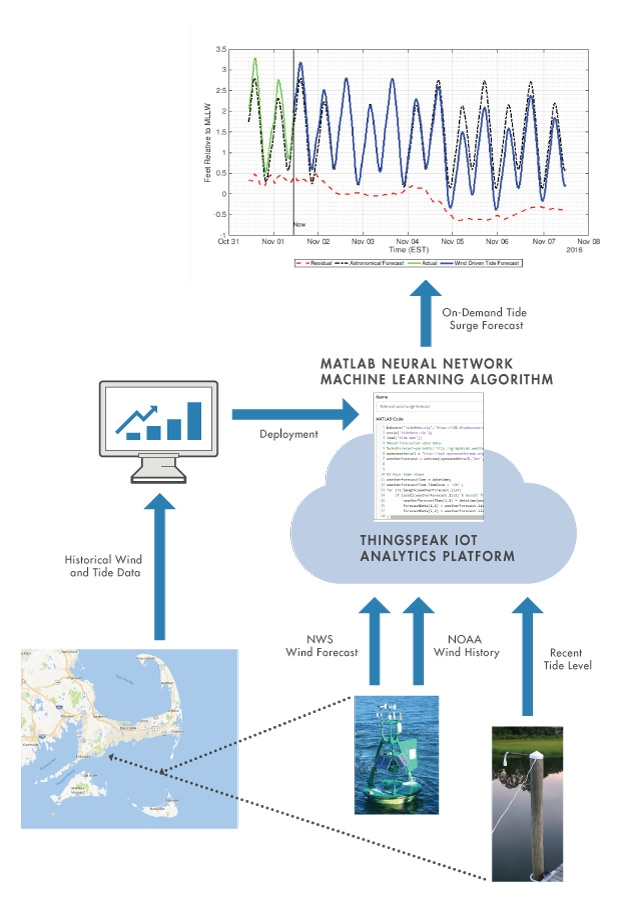
\includegraphics[width=0.5\columnwidth]{images/machine_learning_iot}
	\end{center}
	\caption{Esempio dello sviluppo di un sistema IoT di analisi utilizzando MATLAB, Machine Learning e ThingSpeak \cite{famous:matlab_machine_learning}}
	\label{fig:machine_learning_iot}
\end{figure}
Per soddisfare questa fame di dati e quella che verrà in futuro, per quanto la raccolta dati possa essere automatizzata e distribuita in un numero infinitamente alto di dispositivi, sono necessarie delle risorse ingenti per la distribuzione, manutenzione e creazione di infrastrutture di comunicazione per fare in modo che questi dati siano disponibili ed utilizzabili.
Di qui l'idea del Crowdsourcing di esternalizzare un lavoro o parte di un lavoro ad un gruppo di persone o nel nostro caso, ad un gruppo di cose e persone. L'obiettivo è quello di sfruttare una più grande forza lavoro per il raggiungimento di un certo scopo, ovvero quello della racoclta massiccia di dati. \cite{famous:paper_crowdsourcing_4}
Ricerche dimostrano che ricorrere all'utilizzo del Crowdsourcing, anche al di fuori del mondo IoT, ed in particolare degli approcci di Crowdsourcing legati ai cittadini, possano risultare una fonte affidabile, scalabile e sostenibile per la raccolta di grosse moli di dati. \cite{famous:paper_crowdsourcing_4}
Per chiarire definitivamente il concetto ed i vantaggi del Crowdsourcing, vengono mostrate nella \autoref{sec:crowdsourcing_application} alcune tra le applicazioni più comuni e famose che sfruttano appunto tutta la potenza del Crowdsourcing.

\section{Applicazioni di Crowdsourcing}
\label{sec:crowdsourcing_application}
Attualmente, sono molteplici le applicazioni che sfuttano la potenza messa a disposizione da una \textit{'forza lavoro'} praticamente gratuita ed inesauribile. Queste applicazioni sono talmente comuni ed ottimizzate da non farci nemmeno sospettare di essere noi, con i nostri utilizzi, ad essere la \textit{'forza lavoro'} che produce miliardi di dati e che, molto spesso, quelli stessi dati, dopo opportune analisi, li consuma anche.
Negli esempi contenuti nei paragrafi successivi, sarà subito lampante come queste applicazioni di Crowdsourcing si differenzino principalmente in un aspetto: \textbf{chi genera i dati}. Sono infatti proposte applicazioni nelle quali a generare i dati sono gli umani, condividendo ciò che essi vedono o conoscono. Oppure, ci sono applicazioni nelle quali i dati sono generati dalle macchine, a volte in maniera completamente trasparente all'uomo che spesso ne è addirittura inconsapevole.
\subsection{Google Maps}
Google Maps \textregistered \hspace{2mm} è il celebre servizio offerto da Google che ci consente di orientarci in nuove città, scoprire nuovi posti che potrebbero interessarci, aiutarci a trovare la strada migliore per tornare a casa e guidarci nella navigazione.
Nella fattispecie, il servizio di navigazione offerto da Google Maps \textregistered \hspace{2mm}, si è rivelato ben presto nettamente superiore alle soluzioni di navigazione precedentemente in uso. Questo tutto grazie all'IoT e nella fattispecie ad un sistema di Crowdsourcing tra i più potenti ed avanzati. La feature aggiuntiva di Google Maps \textregistered \hspace{2mm} e di altri servizi simili (Apple Maps \textregistered) sta nel fatto che sono in grado, sulla base della condizione del traffico stimata in real time, di suggerirci la strada migliore per arrivare a casa, in qualsiasi parte del mondo essa sia, nel minor tempo possibile. Per realizzare una simile infrastruttura, sarebbero necessarie centinaia di sensori, sistemi di visione ed antenne per la comunicazione in real time dello stato sul traffico per ogni km di strada, in tutto il mondo. Senza azzardare calcoli, la cifra per la progettazione, sviluppo e manutenzione di un simile impianto sarebbe spropositata persino per Google. Pertanto Google ha deciso di sfruttare il dispositivo IoT più comune, più utilizzato e più diffuso: lo smartphone, lo stesso smartphone che utilizza i servizi offerti da Google Maps \textregistered \hspace{2mm} è utilizzato da Google per ottenere delle stime in real time sul traffico. Di fatto, ogni giorno, miliardi di dispositivi si muovono su tutte le strade del mondo. Questi sono, a tutti gli effetti, dei dispositivi IoT in quanto dotati di sensori, comunicazione attraverso Internet ed una sovrabbondante capacità di calcolo.\\
Non c'è da stupirsi, infatti, se una rete così grande di sensori possa fornire informazioni sufficienti a Google per consigliarci in maniera estremamente accurata di seguire un percorso piuttosto che un altro per tornare a casa evitando così rallentamenti o incidenti.
\begin{figure}
	\begin{center}
		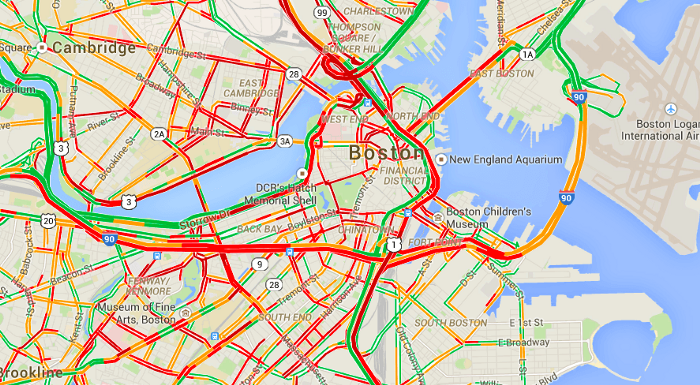
\includegraphics[width=0.7\columnwidth]{images/google_map_traffic}
	\end{center}
	\caption{Indicazione sul livello di traffico stradale nella città di Boston}
	\label{fig:google_map_traffic}
\end{figure}
La capacità di combinare la velocità di un dispositivo con la velocità di altri dispositivi sulle strade, utilizzando migliaia di smartphone in movimento in una area geografica ad un dato periodo di tempo, ha consentito ai servizi offerti da Google di fornire una panoramica affidabile delle condizioni di traffico in real time. Tutto questo ottenuto senza sborsare l'enorme cifra necessaria alla distribuzione di una quantità spropositata di sensori sulla rete stradale di tutto il mondo, ma utilizzando una delle più grandi piattaforme di Crowdsourcing completamente invisibile a coloro che la utilizzano e completamente invisibile a coloro che contribuiscono alla creazione di dati. \cite{patent:google_traffic_info}
\subsection{Linux e Wikipedia}
Un esempio di Crowdsourcing completamente differente da quello mostrato in precedenza, è quello che ha consentito la realizzazione di piattaforme come Wikipedia e del sistema operativo Linux.
In questo caso, infatti, l'utente non solo è consapevole di contribuire alla realizzazione di un progetto distribuito, ma anche deve mettere a disposizione attivamente le proprie competenze per contribuire al progetto.\\
In Wikipedia, ogni utente registrato, è spronato a dare il proprio contributo per l'accrescimento della più grande enciclopedia pubblica e gratuita. La \textit{'forza lavoro'} in questo caso è consapevole del ruolo svolto, della sua importanza e dell'impatto che esso ha sulla comunity di utilizzatori.\\
Allo stesso modo, il sistema operativo Linux, viene sviluppato e manutenuto da una community di sviluppatori, il cui contributo è quello di mettere a disposizione le proprie competenze informatiche per sviluppare e quindi rilasciare il Sistema Operativo in forma Open Source.\\
In entrambi i casi, il sistema Crowdsourcing è stato indispensabile alla creazione del prodotto finito.
Se pensiamo a Wikipedia, in essa sono contenute più di 320 milioni di pagine, tradotte in 280 lingue, uno sforzo immane se questo lavoro fosse toccato ad una sola persona o ad una sola azienda. Invece, sfruttando il Crowdsourcing, si raccoglie tutta la conoscenza acquisita da qualsiasi uomo in qualsiasi parte del mondo, in qualsiasi istante di tempo. \cite{book:wikistats}\\
I numeri di Linux, sono altrettanto impressionanti, si stima infatti che al 2018, Linux fosse composto da oltre 25 milioni di righe di codice, scritte da più di 19 mila diversi contributori. (fonte: \url{https://linux.slashdot.org/})
Ancora una volta, questi numeri sono possibili grazie ad una community che collabora per il raggiungimento di un certo fine che, in questo caso, piuttosto che finalizzato alla raccolta dei dati, è finalizzato alla condivione della conoscenza e delle competenze.

\section{Crowdsourcing ed Internet of Things}
Ora che sono chiare le potenzialità offerte dal Crowdsourcing, è necessario affrontare un altro tema che consentirà di avere una più chiara visione sul legame Crowdsourcing ed IoT dal quale sarà possibile trarre utili informazioni necessarie alla progettazione fatta nel \autoref{chap:tre}.\\
Sebbene evidenti i vantaggi delle piattaforme di Crowdsourcing negli esempi mostrati nella \autoref{sec:crowdsourcing_application}, vanno tuttavia effettuate alcune considerazioni ed accorgimenti da intraprendere quando si utilizzano simili strumenti.\\
Il mondo dell'Internet of Things, si adatta perfettamente a quella che è l'idea alla base del Crowdsourcing : \textit{Esternalizzazione di una parte del lavoro ad un gruppo di persone, le quali, con contributi indipendenti e non organizzati lavorano per uno scopo comune}. Se ci si sforza ad estendere questa definizione non solo alle persone ma anche alle cose, è possibile vedere come questa nuova definizione del Crowdsourcing applicata agli oggetti, bene si adatti con il paradigma dell'Internet of Things.
Se grazie agli strumenti, sensori, protocolli e sistemi integrati offerti dal paradigma IoT è possibile garantire che qualsiasi oggetto possa raccogliere dati e condividerli attraverso Internet, il Crowdsourcing ci suggerisce che tutti questi dati, raccolti come contributi indipendenti da un grande numero di dispositivi, possano essere raggruppati ed utilizzati insieme per il raggiungimento di un più grande scopo. \cite{famous:paper_crowdsourcing_4} \cite{famous:paper_crowdsourcing_2}\\
Nella \autoref{sec:crowdsourcing_application} è stata volutamente omessa una informazione. Sebbene sia vero che senza il Crowdsourcing sarebbe stato impossibile per Linux raggiungere le 25 milioni di righe di codice e per Wikipedia sarebbe stato impossibile raggiungere le 320 milioni di pagine, è anche vero che il contributo dei 19 mila sviluppatori di Linux e dei 4 milioni di utenti registrati in Wikipedia vada gestito e regolamentato. Si rende cioè necessario trovare una sorta di Protocollo o di Interfaccia comune che tutti i contributori, sebbene indipendenti, debbano seguire ed adottare per contribuire al progetto.\\
In Linux questa interfaccia risiede nel software Git per il source control. In questo modo ogni sviluppatore che contribuisce al progetto Linux può clonare \footnote{Termine utilizzato per indicare l'ottenimento di una copia di un progetto globale in una propria cartella locale} o fare un branch \footnote{Termine che indica l'esecuzione di una diramazione di un certo progetto, in un certo stato} del progetto esistente, aggiungere le proprie modifiche ed effettuare nuovamente un commit \footnote{Termine che indica la conferma dell'esecuzione di una modifica ad un dato progetto} sul server così che tutti possano prendere visione delle modifiche apportate. Soltanto dopo aver verificato che le modifiche di un certo utente siano conformi al task richiesto, non introducano problemi o bug e non comportino un rischio per la sicurezza, ne viene effettuato il merge \footnote{Termine che indica l'unione di due versioni dello stesso codice} all'interno della directory principale.\\
Analogamente, in Wikipedia, è necessario verificare la veridicità e la correttezza dei contributi di ciascun utente. A tal proposito, Wikipedia si affida ad un'altra forma di Crowdsourcing, questa volta realizzata non solo da utenti registrati ma anche da coloro che usufruiscono del servizio che possono segnalare argomenti che ritengono sbagliati o non completi.\\
Questa necessità di realizzare una Interfaccia o un Protocollo comune a tutti i contributori di una piattaforma di Crowdsourcing si rende necessaria non solo nelle applicazioni dove i contributori sono umani, ma anche in quelle dove i contributori sono macchine.\\
Come evidenziato nel \autoref{chap:introduzione}, la forza dell'Internet of Things è quella di abilitare una comunicazione ed uno scambio dati tra dispositivi eterogenei. Con eterogenei si intende una differente potenza di calcolo, dotazione sensoristica, funzionamento, costo e casa produttrice. Il risultato di questa eterogeneità è che non esiste un modo comune di identificare un particolare dispositivo all'interno di una piattaforma di Crowdsourcing, ovvero il tipo del dispositivo, il costruttore e quali dati sono prodotti non sono informazioni regolate da uno Standard comune. \cite{famous:paper_crowdsourcing_4} Una difficoltà aggiuntiva se si realizza una piattaforma di Crowdsourcing con dispositivi IoT, sta nel fatto che sia necessario gestire e legittimare l'accesso e la produzione dei dati. Analogamente a quanto fatto da Wikipedia e Linux, è cioè necessario gestire i contributi dei singoli ed ulteriormente verificare che essi siano corretti e conformi.
I problemi legati allo sviluppo di una piattaforma di Crowdsourcing legata a dispositivi IoT sono quindi:
\begin{enumerate}
	\item \textbf{Interoperabilità Semantica :} L'IoT è una tecnologia \textit{'industry driven'} nella quale ogni costruttore realizza la sua piattaforma IoT. In più, la maggior parte delle soluzioni IoT sono case-centric con la conseguente creazione di \textit{'IoT Silos'} i quali, per comunicare tra loro e scambiarsi dati, hanno bisogno di una interoperabilità \textit{'Inter-Silos'}. Si rende necessario che ogni Protocollo o Standard debba considerare la varietà dei dispositivi, il loro contesto di utilizzo ed i dati emessi. La sfida nel dominio IoT è dovuta alla presenza di una varietà di ontologie che trattano vari aspetti dei sensori e delle grandezze da misurare (diversa portata, granularità e generalità). Questo complica lo sviluppo di una ontologia formale o di un Protocollo di comunicazione comune a tutti i dispositivi.
	\item \textbf{Condivisione dei Dati e Controllo degli Accessi :} Un'altra grande sfida per la ricerca nel campo dell'IoT è quella di garantire la privacy degli utenti e la protezione dei dati personali, specialmente in sistemi nei quali si effettua raccolta, gestione e condivisione dei dati. L'identificazione e la gestione di miliardi di dispositivi connessi tra loro ed il mantenimento di una comunicazione affidabile e sicura, rappresentano un punto critico da regolamentare.
	Questo richiede sia lo sviluppo di una policy che regolamenti la comunicazione ma anche richiede uno sviluppo tecnologico per la condivisione sicura ed affidabile con protocolli leggeri ed interoperabili.
	\item \textbf{Elaborazione di Politiche Democratiche :} Alcuni domini specifici nei quali l'IoT si sta diffondendo come l'healthcare e le smart cities, sono campi di applicazione nei quali gli individui operano non soltanto come data providers, ma essi partecipano attivamente nella risoluzione di problemi, condivisione di soluzioni e formulazione di leggi e regolamenti. Si rende quindi necessario adattare il comportamento e i Protocolli o Standard di comunicazione alle particolari politiche democratiche ed ulteriormente al particolare campo di applicazione.
\end{enumerate}






